\section{梯度优化}

% --------------------------------------------------------------------------------------------------------- % 
% 神经网络架构搜索
% --------------------------------------------------------------------------------------------------------- % 
\subsection{神经网络架构搜索}
\subsubsection{参考文章：}
\href{https://arxiv.org/pdf/1806.09055}{\textcolor{blue}{DARTS}}:
\url{https://arxiv.org/pdf/1806.09055}

\subsubsection{相应背景知识：}
神经网络架构搜索(Neural Architecture Search)[NAS]，旨在找到特定任务(如图像识别、语音识别)最优的神经网络架构。
NAS属于自动机器学习(AutoML)的范畴。目标是减少甚至消除需要人工设计网络结构的需求。
原理大致如下：\\
1.搜索空间：定义可能的网络结构选项，包括各种层类型(如卷积层，池化层，全连接层等)，层的数量，连接模式和激活函数等。\\
2.搜索策略：通过某种算法在搜索空间中寻找最优结构(进化算法，基于强化学习的算法，贝叶斯优化，梯度法等)。\\
3.性能评估：对搜索到的网络结构进行训练并评估其性能(准确率，推理时间，模型大小等度量标准)。

\subsubsection{文章主要内容：}

DARTS \cite{liu2018darts} 是在 ICLR 2019 上提出的。
大多数 NAS 算法是使用 RL 算法或 Evolution 算法进行结构搜索，把它们当做 black box 优化问题。
然而这样的话的 search space 是离散的，搜索非常耗时了。
DARTS 试图解决这个问题，提出了一种新的网络搜索算法，它的 search space 是连续的，在搜索过程中它通过在验证集上验证，然后使用梯度下降算法来完成搜索。
实验也表明了 DARTS 进行网络架构搜索的计算开销要比普通网络架构算法小几个量级，但搜索得到的网络结构却仍能和之前 SOTA 算法几乎持平。
同时它的泛化能力也很好，不仅可以用于 CNN 结构的搜索，还可以用于 RNN 结构的搜索。


\textcolor{red}{\textbf{核心目标：}}在保证模型性能的同时，尽可能的降低搜索过程中的成本，同时提升架构的通用性。
\subsubsection{具体方法：}

网络架构搜索算法通常需明确三个核心部分：\textcolor{blue}{搜索空间、搜索策略、性能评估。}

\paragraph{1.Search Space:}
DARTS 中搜索的最小单位也叫 cell，它是一个 DAG，以它为 block 来构建 architecture。
每个 cell 以 N 个有序的 nodes 组成，每个 node $x^{(i)}$ 代表一个 latent representation，每条 edge $(i,j)$ 
代表在 $x^{(i)}$ 执行了某种 operation $o^{(i,j)}$。  
\begin{equation}
	x^{(j)}=\sum_{i<j}o^{(i,j)}\left( x^{(i)} \right).
\end{equation}

\paragraph{2.Continuous Relaxation and Optimization:}
我们用 $\mathcal{O}$ 来表示 candidate operations，到目前为止，search space 还是离散的。所以为了使 search space 连续，作者为 edge 上的每一种 operation 赋上一个 weight $\alpha_0^{(i,j)}$。所以 operation 可表示为：
\begin{equation}
	\hat{o}^{(i,j)}(x) = \sum_{o \in \mathcal{O}} 
	\frac{\exp\left(\alpha_o^{(i,j)}\right)}{\sum_{o' \in \mathcal{O}} 
	\exp\left(\alpha_{o'}^{(i,j)}\right)} o(x)
\end{equation}
其实这也很简单，就是利用 $\alpha = \alpha_o^{(i,j)}$ 做一个 softmax 激活，然后对各种 operation 作加权平均罢了。
那么问题实际上就是被转移成 learn 一组参数 $\alpha = \{\alpha_o^{(i,j)}\}$ 了，
搜索结束后只要通过 $o^{(i,j)} = \arg\max_{o \in \mathcal{O}} \alpha_o^{(i,j)}$ 把 
$\hat{o}^{(i,j)}$ 替换成 $o^{(i,j)}$ 就可以了。下图是一个示意图：
\begin{figure}[H]
	\centering
	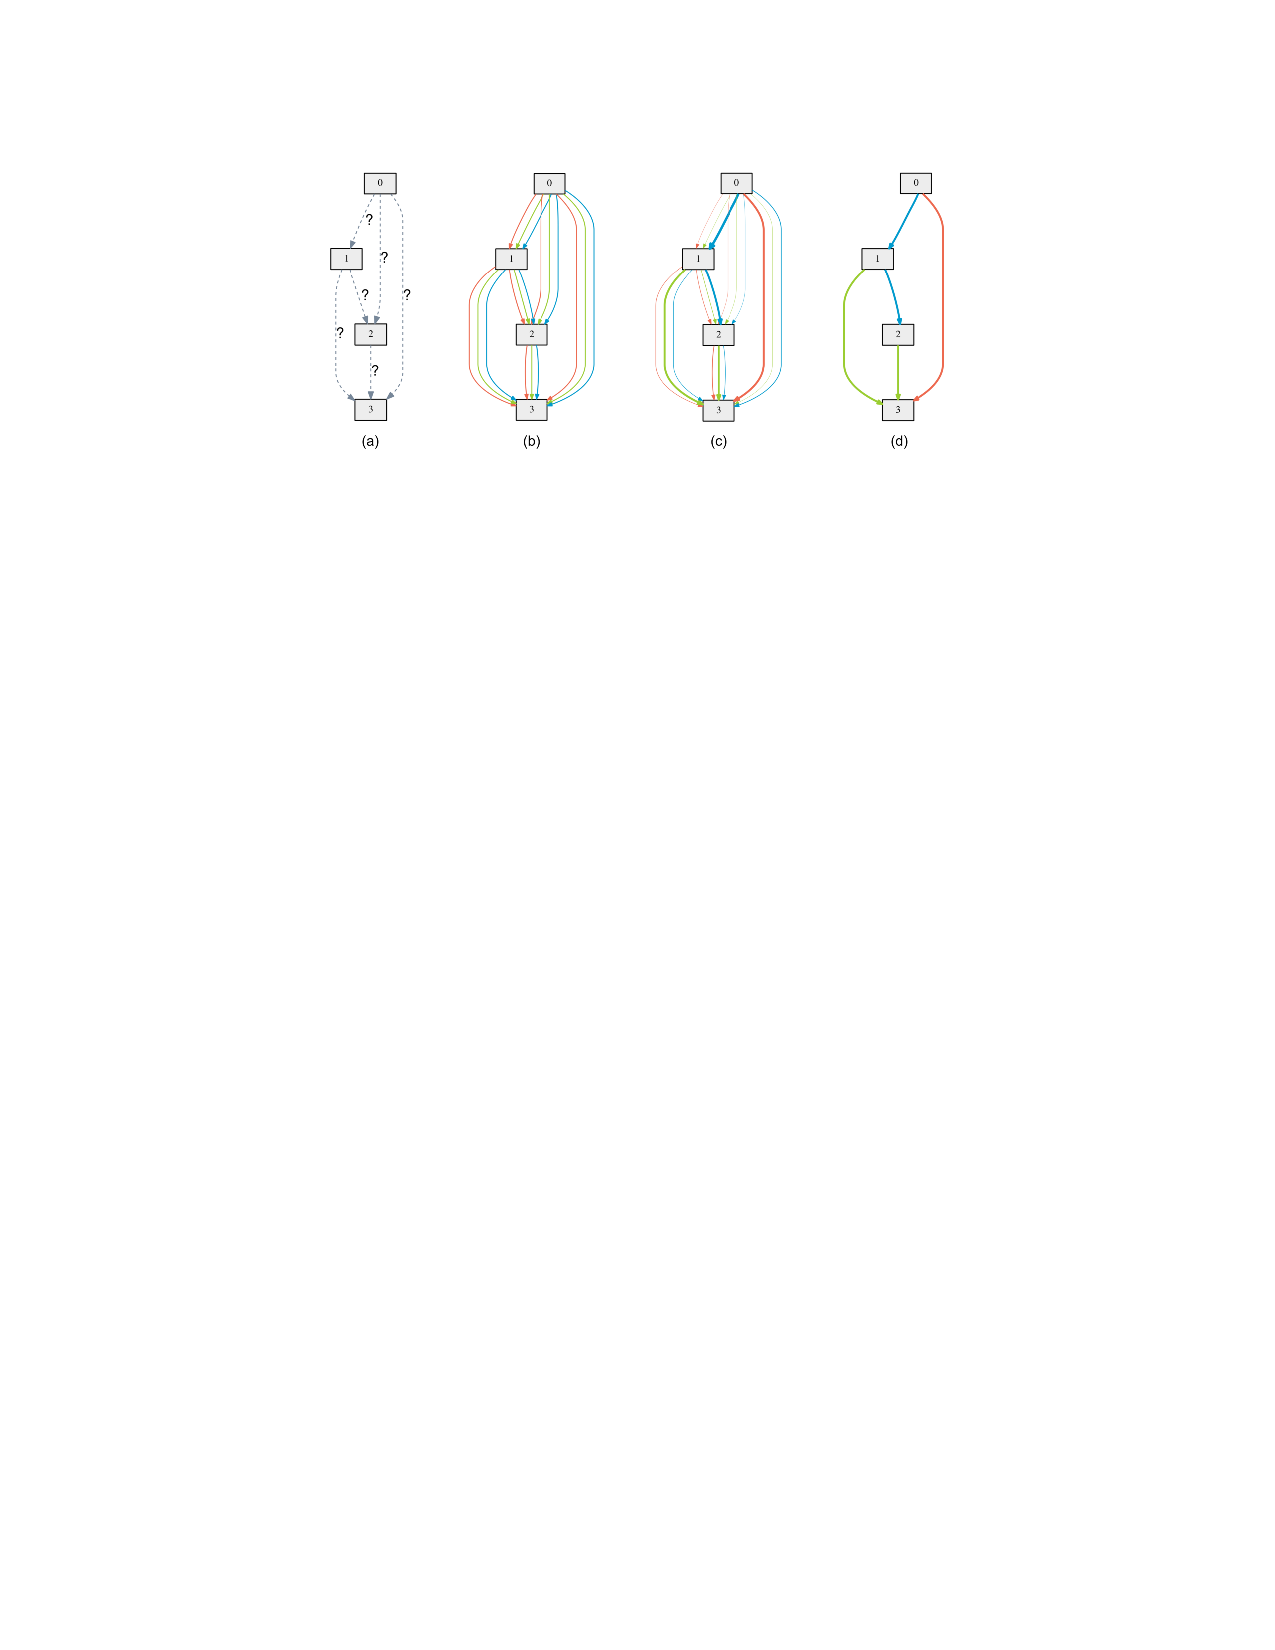
\includegraphics[scale=0.9]{Images/Chapter6_images/DARTS.pdf}
\end{figure}
我们再记具体某个 architecture 里的可训练的 weights 为 \( w \)（e.g. convolution, maxpooling 里的 weights），那么优化问题就变成了最小化验证集上的 loss \( \mathcal{L}_{val}\left(w^*,\alpha^*\right) \)，当 architecture 固定即 \( \alpha^* \) 固定时，需要得到 \( w^* \) 来最小化训练集上的 loss \( w^* = \arg\min_w \mathcal{L}_{train}\left(w,\alpha^*\right) \)。

上述问题，其实就变成了：
\begin{align}\label{eq6:darts}
	\min_{\alpha} \quad & \mathcal{L}_{\text{val}}\left(w^*(\alpha), \alpha\right), \\
	\text{s.t.} \quad & w^*(\alpha) = \arg\min_{w} \mathcal{L}_{\text{train}}(w, \alpha).
\end{align}

这实际上就变成了一个 bilevel optimization 的问题。

\paragraph{3 Approximate Architecture Gradient}

直接去优化 \eqref{eq6:darts} 式比较困难，所以作者采用了迭代近似优化的方法，这也是这篇论文很厉害的地方：

\begin{equation}
	\begin{split}
		\nabla_{\alpha} \mathcal{L}_{\text{val}}\left(w^*(\alpha), \alpha\right) &\approx \nabla_{\alpha} \mathcal{L}_{\text{val}}\left(w - \xi \nabla_w \mathcal{L}_{\text{train}}(w, \alpha), \alpha\right).
	\end{split}
\end{equation}

其中 $\xi$ 是学习率，上式其实是一个复合函数求导，进一步展开化简为：

\begin{equation}
	\nabla_{\alpha} \mathcal{L}_{\text{val}}\left(w', \alpha\right) - \xi \nabla_{\alpha,w}^2 \mathcal{L}_{\text{train}}(w, \alpha) \nabla_w \mathcal{L}_{\text{val}}\left(w', \alpha\right).
\end{equation}

接着利用泰勒展开进一步化简得到：

\begin{equation}
	\nabla_{\alpha,w}^2 \mathcal{L}_{\text{train}}(w, \alpha) \nabla_w \mathcal{L}_{\text{val}}\left(w', \alpha\right) \approx \frac{\nabla_{\alpha} \mathcal{L}_{\text{train}}\left(w^+, \alpha\right) - \nabla_{\alpha} \mathcal{L}_{\text{train}}\left(w^-, \alpha\right)}{2\epsilon}.
\end{equation}

\subsubsection{总结}
文章的核心思想的简要流程：
\begin{enumerate}
	\item 将网络的不同层，不同模块包装成一个cell
	\item 对每个cell之间进行权重连接
	\item 训练结合问题的目标函数，优化权重参数
	\item 得到最合适的结构
\end{enumerate}















